\documentclass{beamer}
\usetheme[%
 titleformat=allcaps,%
 block=fill,%
 % background=dark,%
 progressbar=foot,%
 subsectionpage=progressbar,%
 numbering=none%
]{Metropolis}
\setbeamertemplate{%
 navigation symbols%
}{} % suppresses all navigation symbols
\usepackage{listings}
\usepackage{xcolor}
\usepackage{graphicx}
\definecolor{monsanto}{RGB}{00,88,56}
\setbeamercolor{normal text}{fg=monsanto, bg=white}

\lstset{language=HTML}

\renewcommand{\arraystretch}{1.5}

\begin{document}
\title{Intro to HTML}
\author{Artem Chernyak}

\frame{\titlepage}

\AtBeginSection[]{
  \begin{frame}
    \frametitle{Table of Contents}
    \tableofcontents[currentsection]
  \end{frame}
}

\section[Section]{Markup}

\begin{frame}
  \frametitle{Definition}
  A system for annotating a document in a way that is syntactically
  distinguishable from the text.
\end{frame}

\begin{frame}
  \frametitle{Markdown}
  \begin{columns}
    \column {.5\textwidth}
    \# Hello\\
    \bigskip
    * Easy\\
    * Formatting\\
    \column {.5\textwidth}
    {\huge Hello}
    \begin{itemize}
      \item Easy
      \item Formatting
    \end{itemize}
  \end{columns}
\end{frame}

\begin{frame}
  \frametitle{Importance}
  \begin{itemize}
    \item separates content and layout
    \item easy to share
    \item edito agnostic
    \item universaly understood
  \end{itemize}
\end{frame}

\section[Section]{HTML Structure}

\begin{frame}
  \frametitle{Intro}
  \begin{itemize}
    \item markup lanugage
    \item designed to display text documents
    \item supports almost no styling without css
    \item most used markup language in teh world
  \end{itemize}
\end{frame}

\begin{frame}
  \frametitle{Anatomy of an HTML element}
  \begin{center}
    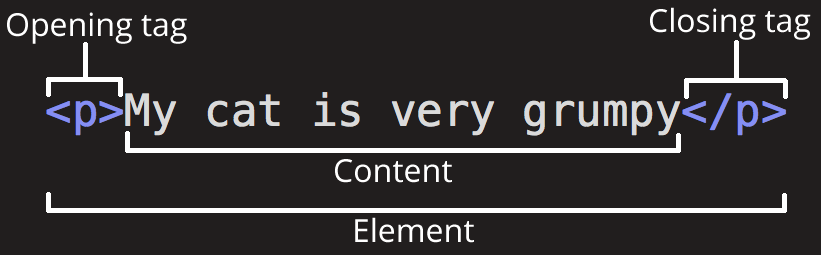
\includegraphics[scale=.35]{html-element.png}
  \end{center}
\end{frame}

\begin{frame}
  \frametitle{Block elements}
  \begin{itemize}
    \item appear on new line
    \item following element will be on a new line
    \item structure elements
    \item can appear nested inside each other
    \item should not be nested inside an inline element
  \end{itemize}
\end{frame}

\begin{frame}
  \frametitle{Inline element}
  \begin{itemize}
    \item does not start a new line
    \item used to surround small parts of a document
    \item normally inside paramgraphs of text
  \end{itemize}
\end{frame}

\begin{frame}[fragile]
  \frametitle{Element types example}
  \begin{columns}
    \column {.5\textwidth}
    \begin{lstlisting}
      <em>first</em>
      <em>second</em>
      <em>third</em>
      <p>fourth</p>
      <p>fifth</p>
      <p>sixth</p>
    \end{lstlisting}
    \column {.5\textwidth}
    \textit{firstsecondthird}\\
    fourth\\
    fifth\\
    sixth
  \end{columns}
\end{frame}

\begin{frame}
  \frametitle{Attributes}
  \begin{center}
    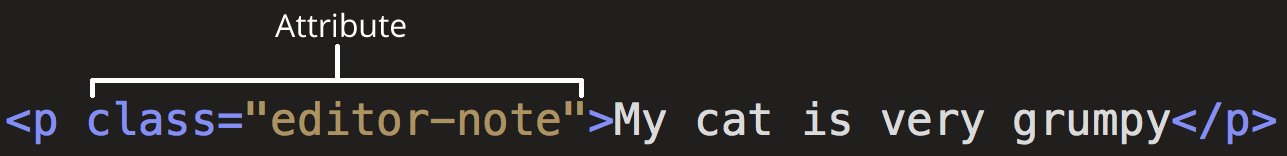
\includegraphics[scale=.25]{attribute.png}
  \end{center}
\end{frame}

\begin{frame}[fragile]
  \frametitle{Whitespace}
  \begin{columns}
    \column {.5\textwidth}
    \begin{lstlisting}[basicstyle=\footnotesize]
      <p>Dogs are silly.</p>
    \end{lstlisting}
    \column {.5\textwidth}
    \begin{lstlisting}[basicstyle=\footnotesize]
      <p>Dogs        are
         silly.</p>
    \end{lstlisting}
  \end{columns}
\end{frame}

\section[Section]{Block elements}

\begin{frame}[fragile]
  \frametitle{Paragraph}
  \begin{lstlisting}
    <p>Hello class</p>
  \end{lstlisting}
  \begin{itemize}
    \item block element
    \item used to wrap paragraphs of text
    \item no other properties
  \end{itemize}
\end{frame}

\begin{frame}[fragile]
  \frametitle{Headings}
  \begin{lstlisting}
    <h1>Hello</h1>
  \end{lstlisting}
  \begin{itemize}
    \item used to wrap text
    \item makes test bigger and bolder than standard
    \item \begin{lstlisting}[basicstyle=\small]
<h1>,<h2>,<h3>,<h4>,<h5>,<h6>
    \end{lstlisting}
  \end{itemize}
\end{frame}

\begin{frame}[fragile]
  \frametitle{Unorderd List}
  \begin{lstlisting}
    <ul>
      <li>One</li>
      <li>Two</li>
    </ul>
  \end{lstlisting}
  \begin{itemize}
    \item block element
    \item creates a bullet point list
    \item each of the elments should have an \textit{li}
  \end{itemize}
\end{frame}

\begin{frame}[fragile]
  \frametitle{Ordered List}
  \begin{lstlisting}
    <ol>
      <li>One</li>
      <li>Two</li>
    </ol>
  \end{lstlisting}
  \begin{itemize}
    \item block element
    \item creates a numbered list
    \item each of the elments should have an \textit{li}
  \end{itemize}
\end{frame}

\section[Section]{Inline elements}

\begin{frame}[fragile]
  \frametitle{Italicize and bold}
  \begin{lstlisting}
    <em>Hello</em><strong>World</strong>!!!
  \end{lstlisting}
  \begin{itemize}
    \item inline elements
    \item \textit{em} will make the contents italicized
    \item \textbf{strong} will make the contents bold
  \end{itemize}
\end{frame}

\begin{frame}[fragile]
  \frametitle{Link}
  \begin{lstlisting}[basicstyle=\footnotesize]
    <a href="http://test.com"
        title="Test link">Sample link</a>
  \end{lstlisting}
  \begin{itemize}
    \item inline element
    \item turns anything inside into a clickable link
    \item href is required provide a url
    \item can contain other elements
    \item title is used to show hover text
  \end{itemize}
\end{frame}

\begin{frame}[fragile]
  \frametitle{Images}
  \begin{lstlisting}[basicstyle=\footnotesize]
    <img src="test.png" alt="test image">
  \end{lstlisting}
  \begin{itemize}
    \item inline element
    \item displays the provided image
    \item src is the relative path to an image
    \item alt will display text if no image found
  \end{itemize}
\end{frame}

\section[Section]{Non-sementic Elements}

\begin{frame}
  \frametitle{Definition}
  \begin{itemize}
    \item elements with no meaning
    \item only use if no other element can be used
    \item can be used for grouping and placement
  \end{itemize}
\end{frame}

\begin{frame}[fragile]
  \frametitle{Div}
  \begin{lstlisting}[basicstyle=\footnotesize]
    <div>
      <p>This div is useless</p>
    </div>
  \end{lstlisting}
  \begin{itemize}
    \item block element
    \item used in advanced layouts
    \item can be used to group and change style of large areas of text
  \end{itemize}
\end{frame}

\begin{frame}[fragile]
  \frametitle{Span}
  \begin{lstlisting}[basicstyle=\footnotesize]
    <p>This span is <span>useless</span></p>
  \end{lstlisting}
  \begin{itemize}
    \item inline element
    \item used for highly customized text elements
    \item only use if no other inline elment makes sense
  \end{itemize}
\end{frame}

\section[Section]{Most important attributes}

\begin{frame}[fragile]
  \frametitle{Images}
  \begin{lstlisting}[basicstyle=\footnotesize]
    <div class="custom-layout">
      <p>This is how you make a useful</p>
    </div>
  \end{lstlisting}
  \begin{itemize}
    \item used to apply style to multiple elements
    \item can contain multiple style
    \item the same elment can be applied to multple elements
    \item should be most commonly used attribute for styling
  \end{itemize}
\end{frame}

\begin{frame}[fragile]
  \frametitle{Images}
  \begin{lstlisting}[basicstyle=\footnotesize]
    <div id="custom-layout">
      <p>This is how you make a useful</p>
    </div>
  \end{lstlisting}
  \begin{itemize}
    \item used for a single special element
    \item can contain multiple style
    \item the same id should never be reused
  \end{itemize}
\end{frame}
\end{document}
